\chapter{Governing Equations and the Numerical Model}
Here in this chapter of the report, we summarize the governing equations of heat transport processes inside and around the Borehole Heat Exchangers (BHEs).  Also, the details of this mathematical formulation and the techniques applied to solve it numerically will be discussed. Note that the method implemented here is not the creative work of the authors, but rather a collection of contributions from the scientific community. The formulation of heat exchange between BHEs and the surrounding soil, was proposed by Al-Khoury et al \cite{AlKhoury2010}. This formulation was later-on adopted by Diersch et al. \cite{Diersch2011a} \cite{Diersch2011b} into the commercial software FEFLOW. In this work, we followed the same idea as Al-Khoury and Diersch, and implemented the heat transport process in response to BHEs into the open-source scientific software OpenGeoSys. For interested readers, the FEFLOW book \cite{FEFLOW2014} also serves a good reference for the better understanding of this work. 
%%
\begin{figure}
\begin{center}
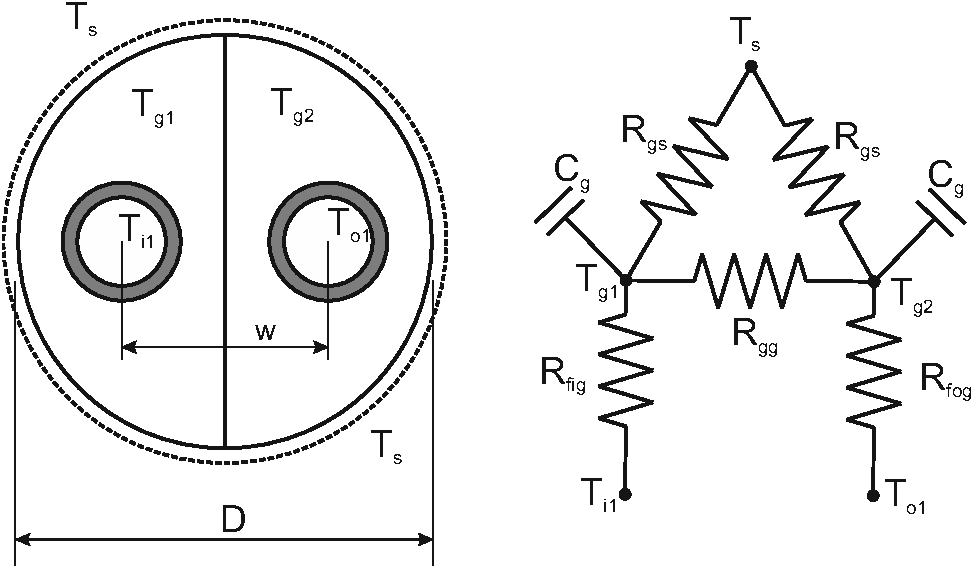
\includegraphics[width=0.8\textwidth]{fig/crosssection_1U}
\end{center}
\caption{Configuration of the 1U type BHE and its corresponding resister-capacitor concept (Reproduced after the FEFLOW book \cite{FEFLOW2014})}
\label{fig:cross_sec_1u}
\end{figure}
%%
\section{Model Concept for BHEs}
To exchange heat with the surrounding soil and rock, borehole heat exchangers have different designs and configurations. The most popular designs can be categorized into 4 differnt types, i.e. the 1U, 2U, CXC and CXA. The U-type BHEs are named after the U shaped tubes laid vertically along the borehole. The number 1 or 2 refer to how many pairs of U tubes are in the same borehole. To illustrate this, Fig \ref{fig:cross_sec_1u} shows the horizontal cross-section of a 1U type BHE. Notice that the U tubes are normally sealed by grout materials, and not in direct contact with the soil. For a typical BHE, a refrigerant fluid is circulating inside of the U tube, absorbing or releasing heat into the surrounding grout and soil. 
%%
In order to numerically simulate the heat transfer inside of a BHE, the device is further conceptualized by the so-called Resister-Capacitor model. This idea originates from the electrical engineering field. In a electrical circuit, if the electric current is hindered by a component, we call this component a Resistor. When a component is capable of storing the electricity, we call it a Capacitor. So the same concept is also applied to the heat transport process in a BHE. Taking the 1U type of BHE in Figure X as an example, there are 4 temperature values assigned to a BHE cross-section at a particular depth. They are $T_s$, $T_{i1}$, $T_{o1}$, $T_{g1}$ and $T_{g2}$, referring to the temperatures of the surrounding soil, the inlet pipe, the outlet pie, the 1st and the 2nd grout zone respectively. As a convention, we always assume the 1st grout zone is the one surrounding the inlet pipe. Following this concept, the heat transfer between the pipe and the soil can be divided into five pathways: i) between inlet pipe and 1st grout zone; ii) between outlet pipe and 2nd grout zone; iii) between 2 grout zones; iv) between 1st grout zone and the soil; v) between 2nd grout zone and the soil. The heat flux $q_n$ on each of these pathways, are driven by the temperature difference and regulated by the heat transfer coefficient $\Phi$. For example, the heat flux from inlet pipe to the 1st grout zone can be calculated by 
\begin{equation}
q_n = \Phi_{fig} \left( T_{i1} - T_{g1} \right), 
\end{equation} 
which is inversely dependent on the product of heat resistance $R$ and specific exchange area $S$
\begin{equation}
\Phi = \frac{1}{R S}
\end{equation}
Depending on the different pathways, we have corresponding heat transfer coefficients, denoted as $\Phi_{fig}$, $\Phi_{fog}$, $\Phi_{gg}$ and $\Phi_{gs}$.  
~~\
\section{Governing Equations}
\subsection{Governing Equations for the Heat Transport Process in Soil}
For the heat transport process in the soil, the development of soil temperature $T_s$ is contributed by both the heat convection of the fluid $f$ in the soil and the heat conduction through the soil matrix. Let $\rho^s$, $\rho^f$ and $c^s$, $c^f$ be the density and specific heat capacity of fluid $f$ and soil $s$. If assuming the soil matrix is fully saturated with groundwater, the Darcy velocity of which is described by the vector $q$, then the conservation equation writes as
\begin{equation}
\frac{\partial}{\partial t}  \left[ \epsilon \rho^f c^f + ( 1-\epsilon ) \rho^s c^s \right]  T_s 
+ \nabla \cdot \left(  \rho^f c^f \bf{q} T_s  \right) 
- \nabla \cdot \left(  \Lambda^s \cdot \nabla T_s  \right) = H_s,  
\end{equation}
with $\Lambda^s$ the tensor of thermal hydrodynamic dispersion and $H_s$ the source and sink terms for heat. When considering the heat exchange between the BHEs and the soil, the above governing equation is subject to a Cauchy-type of boundary condition: 
\begin{equation}
- \left(  \Lambda^s \cdot \nabla T_s  \right) = q_{n T_s}. 
\end{equation}


\subsection{Governing Equations for the Borehole Heat Exchangers}


\section{Numerical Model}

\subsection{Mesh Arrangement}

\subsection{Finite Element Discretization}

\subsection{Assembly of the Global Equation System}

\subsection{Picard Iterations and Time Step Schemes}